\documentclass[12pt]{article}
\linespread{1.6}

\usepackage{amsmath}
\usepackage{amssymb}
\usepackage{graphicx}
\graphicspath{{images/}}
\usepackage{indentfirst}
\usepackage{lipsum}
\usepackage{xcolor}
\usepackage{soul}
\usepackage{setspace}
\usepackage[
backend=biber,
style=alphabetic,
sorting=ynt
]{biblatex}
\usepackage{hyperref}
\usepackage{tikz}
\usetikzlibrary{shapes.geometric, positioning, fit, arrows.meta}

%-----------some colors
\newcommand{\standardcolor}{blue}
\newcommand{\unlimicolor}{red}
\newcommand{\combcolor}{green}

\tikzstyle{startstop} = [rectangle, rounded corners, 
minimum width=3cm, 
minimum height=1cm,
text centered, 
draw=black, 
fill=\standardcolor!30]

\tikzstyle{combFn} = [trapezium, 
trapezium stretches=true, % A later addition
trapezium left angle=70, 
trapezium right angle=110, 
minimum width=3cm, 
minimum height=1cm, text centered, 
draw=black, fill=\combcolor!50,
rounded corners]

\tikzstyle{unlimiFn} = [trapezium, 
trapezium stretches=true, % A later addition
trapezium left angle=70, 
trapezium right angle=110, 
minimum width=3cm, 
minimum height=1cm, text centered, 
draw=black, fill=\unlimicolor!50,
rounded corners]

\tikzstyle{standardFn} = [trapezium, 
trapezium stretches=true, % A later addition
trapezium left angle=70, 
trapezium right angle=110, 
minimum width=3cm, 
minimum height=1cm, text centered, 
draw=black, fill=\standardcolor!50,
rounded corners]

\tikzstyle{process} = [rectangle, 
minimum width=3cm, 
minimum height=1cm, 
text centered, 
text width=3cm, 
draw=black, 
fill=orange!30]
\tikzstyle{decision} = [ellipse, rounded corners,
minimum width=3cm, 
minimum height=1cm, 
text centered, 
draw=black, 
fill=\standardcolor!30]
\tikzstyle{arrow} = [thick,->,>=stealth]
%\usepackage{endfloat}
\addbibresource{sections/references.bib}
\singlespacing
\addtolength{\oddsidemargin}{-.5in}
\addtolength{\evensidemargin}{-.5in}
\addtolength{\textwidth}{1in}

\addtolength{\topmargin}{-.5in}
\addtolength{\textheight}{1in}

\DeclareMathOperator{\softmax}{softmax}
%-----------------------------------------------------------

\begin{document}
%\begin{titlepage}
\begin{center}
\large
\textbf{Project Proposal}\\
\Large
\textbf{Long Document Summarization:}\\
\textbf{Augmenting Unlimiformer with Knowledge Graphs\footnote{\today}}\\
\begin{table}[h]
    \centering
    \begin{tabular}{ccc}
        Patrick O'Callaghan&  Sheel Sansare& Tristan Wang\\
         (patocal)& (ssansa2)  & (aawang99)\\
    \end{tabular}
%    \caption{Caption}
    \label{tab:my_label}
\end{table}
\end{center}
%\end{titlepage}

In this blog post, we explore how knowledge graphs (KGs) can be applied to improve the accuracy of the \texttt{unlimiformer} long-range transformer for the task of long document (LD) summarization.
\section*{Dataset}
We choose to use the Hugging Face versions of the  GovReport 
\cite{huang2021efficient} and BookSum \cite{kryscinski2021booksum} (fullbook)
datasets because they are well-established long-document summarization datasets
that are both publicly available and ready-to-use. The \texttt{unlimiformer}
paper also works with these datasets and our first task is to replicate their
results on these two datasets. Our main focus is GovReport because it is the
larger dataset and it has many real-world applications. We also choose BookSum
not only because it contains longer documents, but also because it is easy to
subjectively judge the quality of a summary for books that we have read before.
The Hugging Face GovReport dataset has an approximate $90/5/5\%$ split of
approximately $19.5$k document-summary pairs. The full-book BookSum dataset
has an approximate $80/10/10\%$ split of just over 400 document-summary pairs. 

\section*{Metrics}
We will use ROUGE-1 (unigram), ROUGE-2 (bigram), ROUGE-L (sub-sequence), and BERTScore. The ROUGE metrics are a standard way of comparing summarization performance through lexical overlap between the model-generated and gold summaries. Similarly, the BERTScore is a standard way to compare the semantic similarity between the model-generated and gold summaries by comparing BERT embeddings of both summaries. 
%In summarization tasks, relying solely on lexical similarity might lead to summaries that replicate the source's words but miss its overall meaning. Conversely, only considering semantic similarity might generate summaries that capture the gist but omit specific, crucial details. Using both provides balance.
\section*{Baseline \texttt{unlimiformer} Model}

Since Vaswani et al 2017, transformers have become the default approach to
natural language processing. Transformers have succeeded due to their ability
to capture long range dependencies between tokens. They do so by abandoning the
sequential approach of recurrent neural networks and instead allowing the
decoder to attend to a complete graph over the encoded hidden states. However,
the complexity of complete graphs is quadratic in the number of tokens and this
explains why LLMs have relatively small context windows. 


To bypass this constraint, numerous creative approaches have been proposed and
most involve breaking the document into chunks of size $k$, where $k$ is equal
to the context window length. Our baseline model \texttt{unlimiformer} (see
figure \ref{fig-latex}) bypasses this constraint by changing the contents of
the context window. That is, instead of passing the next chunk of text in the
sequence, it feeds the decoder the $k$-nearest neighbors that it can find in a
datastore that contains all the tokens in the entire document. Consider a
simplified equation of attention \[\text{Attn}(Q, K, V) = \softmax (Q K^T) V,\]
where, for each hidden-layer state $h_d$ of the decoder and the final-hidden
layer state $h_e$ of the encoder,  $Q = h_d W_Q$, $K = h_e W_K$ and $V = h_e
W_v$.\footnote{In the context of translation, think of $h_d$ as the hidden
  state of tokens in ``I am a student” and $h_e$ as the hidden state of tokens
in ``Je suis \'{e}tudiant’’.} The trick is to rewrite  \[(Q K ^T)_{i, j} =
\langle p_{d,i}, h_{e, j}\rangle\] where $p_{d, i} = h_{d, i} W_Q W_K^T$.
This allows us to create a datastore  $\{h_{e, j} \in \mathcal H_{\text{enc}}
: j \in \text{LongDoc}\}$ and identify the $k$ nearest neighbors in the
datastore to the  projection $p_d$. Only those $k$ nearest neighbors are
passed to the decoder of an otherwise standard LLM.

%Let's consider ``je suis \'{e}tudiant" which has 4 tokens and its translation ``I am a student," which also has 5 tokens. We will walk through the dimensions using these specific lengths for clarity. Assume that we're using a single attention head and a batch size of 1, as you specified.
%
%Notation:
%
%- \( Q \) (Query): Generated from the decoder's hidden state \( h_d \).
%- \( K \) (Key), \( V \) (Value): Generated from the encoder's hidden state \( h_e \).
%- \( d_k \): Dimension of the Key (also the dimension of the Query).
%- \( h_d \) and \( h_e \): Hidden states from the decoder and encoder respectively.
%- \( W_q, W_k \): Weight matrices for Query and Key.
%
%Terms Explained:
%
%1. \( h_e \): The hidden state vector for each word in the input sentence, generated by the encoder. For ``je suis étudiant," the encoder produces 4 hidden state vectors, one for each token.
%
%2. \( Q, K, V \): 
%    - \( Q \) is calculated from the decoder's hidden state \( h_d \) using the weight matrix \( W_q \).
%    - \( K \) and \( V \) are calculated from the encoder's hidden state \( h_e \) using the weight matrices \( W_k \) and \( W_v \).
%
%Dimensionality:
%
%Let's consider \( d_k = 64 \) and \( \text{hidden\_dim} = 128 \) as examples.
%
%1. Hidden State Dimensions:
%    - \( h_d \) for ``I am a student" has dimensions \( (1, 5, 128) \).
%    - \( h_e \) for ``je suis étudiant" has dimensions \( (1, 4, 128) \).
%
%2. Weight Matrix Dimensions:
%    - \( W_q, W_k, W_v \) have dimensions \( (128, 64) \).
%
%3. Calculate \( Q, K, V \):
%    - \( Q = h_d W_q \)  \( (1, 5, 128) \times (128, 64) = (1, 5, 64) \)
%    - \( K = h_e W_k \)  \( (1, 4, 128) \times (128, 64) = (1, 4, 64) \)
%    - \( V = h_e W_v \)  \( (1, 4, 128) \times (128, 64) = (1, 4, 64) \)
%
%4. Calculate \( Q K^T \):
%    - \( Q K^T \) will have dimensions \( (1, 5, 4) \).
%
%5. Scale and Apply Softmax:
%    - \( Q K^T / \sqrt{64} \)  dimension remains \( (1, 5, 4) \)
%    - Softmax applied to last axis: \( \text{softmax}(Q K^T / \sqrt{64}) \)  dimension remains \( (1, 5, 4) \).
%
%6. Calculate \( \text{Attn}(Q, K, V) \):
%    - \( \text{softmax}(Q K^T / \sqrt{64}) \times V \)  \( (1, 5, 4) \times (1, 4, 64) = (1, 5, 64) \)
%
%So, the output \( \text{Attn}(Q, K, V) \) will have dimensions \( (1, 5, 64) \), aligning with the sequence length of the decoder output ``I am a student" and the dimension \( d_k \).

\section*{Augmenting \texttt{unlimiformer} with Knowledge Graphs}  Our goal is
to enrich \texttt{unlimiformer} approach with a knowledge graph (see figure
\ref{fig-latex}). To do so, we will use standard entity-extraction techniques
to identify key entities in each document (as in \cite{wu2020extracting}).
Since KGs store richer information than a plain datastores, we aim to show that
they enable us to generate more accurate and coherent summaries. We draw
inspiration from \cite{wang2022multi} in the related task of multi-document
summarization.

Our second step will be to identify an isomorphism between entities $E$ in the
KG and sets $H_{e, E}$ of top-level encodings of tokens (similar to
\cite{galkin2021nodepiece}). For example, if the
literary character $E = \texttt{Karamazov}$, then our entity embedding is the
set $H_{e, E} = \{h_\texttt{Kar}, h_\texttt{amaz}, h_\texttt{ov}\}$ in
$\mathcal H_\text{enc}$. This set of tokens would form a clique in our encoding
of the KG. Relations or edges may also be encoded as sequences of tokens that
connect entities. We recognize that there are still some modelling choices to
be explored in this respect. Yet this perspective of cliques as entities
already brings to mind the \texttt{struct2vec} notion of structural similarity.

Introducing KGs will thus allow us to employ more refined notions of
$k$-``nearest''. In terms of our earlier mathematical discourse,
\texttt{unlimiformer} defines ``nearest’’ according to the topology generated
by the linear functional $\langle p_{d, j}, \cdot \rangle : \mathcal
H_\text{enc} \rightarrow \mathbb R$ for each token $j$ in the target sequence.
This is the \emph{weak topology} over the hidden state space. We will explore
more graph-based topologies such as  structural similarity (in the spirit of
\texttt{struct2vec} \cite{ribeiro2017struc2vec}) which may be more appropriate
for long document summarization.

%We intend to leverage our relative abundance of encoded information (compared to a datastore) to make more intelligent selections of $h_e$ vectors than the baseline model, and in turn produce better long document summaries.
%As with the baseline model, we define $h_d$ as the decoder hidden state and $h_e$ as the encoder's last-layer hidden state.
%For our combined model, instead of storing the hidden-state $h_e$ in a datastore during the encoding process, we will store them as entities in a (hidden representation of a) KG (see Fig. 2). Relations between the entities will be defined by the degree of similarity between the $h_e$ vectors. As such, the KG created will be a hidden KG whose information is only meaningful to the model.
%
%To populate the KG, we propose a TransR model, which models both entities and relations as vectors (say, in $\mathbb{R}^i$ and $\mathbb{R}^j$ space, respectively), with $M \in \mathbb{R}^{j \times i}$ space as the projection matrix and the score function being $f_r(h, t)=-||h_{\perp}+r-t_{\perp}||$. TransR is beneficial since it is capable of encoding symmetric, antisymmetric, inverse, transitive, and $1$-to-N relations.
%

\appendix
\section{Diagram of the combined model}
%\begin{figure}[ht]
%    \centering
%    \includegraphics[scale=.27]{images/baselinemodel_2.png}
%    \caption{The baseline \texttt{unlimiformer} model}
%    \label{fig:baseline}
%\end{figure}
\begin{figure}[ht]
  \centering 
  \vskip.5cm
  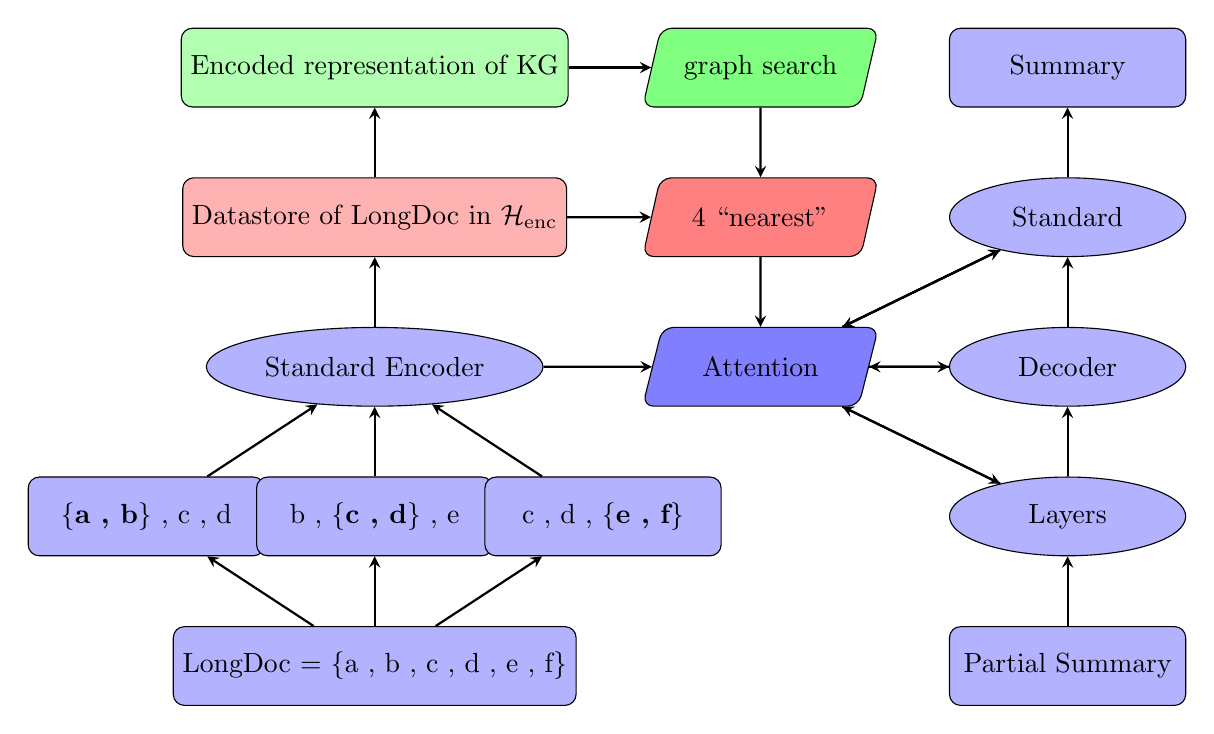
\begin{tikzpicture}[node distance=1.9cm]

%-----------chunks
  \node (chunk1) [startstop] {\{{\bf a , b}\} , c , d};
  \node (chunk2) [startstop, right of=chunk1, xshift=1cm] {b , \{{\bf c , d}\} , e};
  \node (chunk3) [startstop, right of=chunk2, xshift=1cm] 
    {c , d , \{{\bf e , f}\}};
%-----------the long document
\node[draw, rectangle, minimum width=4cm, minimum height=1cm,
  below of=chunk2]
  (longdoc) [startstop]{LongDoc = \{a , b , c , d , e , f\}};
%-----------the encoder
\node (encoder)[decision, above of=chunk2, xshift=0cm] {Standard Encoder};

%-----------the attention mechanism
\node (attn) [standardFn, right of=encoder, xshift=3cm] {Attention};

%-----------unlimiformer-----------
%-----------the datastore
\node[draw, rectangle, fill=red!30, minimum width=4cm, minimum height=1cm,
  above of=encoder, xshift=0cm, rounded corners]
  (datastore) {Datastore of LongDoc in $\mathcal H_\text{enc}$};
%-----------selecting the k nearest
\node (nearest) [unlimiFn, above of=attn] {$4$ ``nearest''};

%-----------combined model
\node[draw, rectangle, fill=green!30, minimum width=4cm, minimum height=1cm,
  above of=datastore, rounded corners]
  (kg) {Encoded representation of KG
%    $2^{\mathcal H_\text{enc}} \times 2^{\mathcal H_\text{enc}}$
  };
%-----------the alternative search
\node (search) [combFn, above of=nearest] {graph search};
%

%-----------decoder
\node (decoder2) [decision, right of=attn, xshift=2cm, yshift=0cm]
  {Decoder};
%-----------decoder
\node (decoder1) [decision, below of=decoder2]
  {Layers};
%-----------decoder
\node (decoder3) [decision, above of=decoder2]
  {Standard};

%-----------partial summary
\node (parsum) [startstop, below of=decoder1] {Partial Summary};
%-----------final summary
\node (sum) [startstop, above of=decoder3] {Summary};

\draw [arrow] (longdoc) -- (chunk1);
\draw [arrow] (longdoc) -- (chunk2);
\draw [arrow] (longdoc) -- (chunk3);
\draw [arrow] (chunk1) -- (encoder);
\draw [arrow] (chunk2) -- (encoder);
\draw [arrow] (chunk3) -- (encoder);
\draw [arrow] (encoder) -- (datastore);
\draw [arrow] (datastore) -- (kg);
\draw [arrow] (datastore) -- (nearest);
\draw [arrow] (kg) -- (search);
\draw [arrow] (search) -- (nearest);
\draw [arrow] (nearest) -- (attn);
\draw [arrow] (decoder1) -- (attn);
\draw [arrow] (decoder2) -- (attn);
\draw [arrow] (decoder3) -- (attn);
\draw [arrow] (attn) -- (decoder3);
\draw [arrow] (attn) -- (decoder1);
\draw [arrow] (attn) -- (decoder2);
\draw [arrow] (attn) -- (decoder3);
\draw [arrow] (encoder) -- (attn);
\draw [arrow] (parsum) -- (decoder1);
\draw [arrow] (decoder1) -- (decoder2);
\draw [arrow] (decoder2) -- (decoder3);
\draw [arrow] (decoder3) -- (sum);

\end{tikzpicture}
\caption{\footnotesize A stylised transformer with length-$4$ context window
  (in blue).  The standard approach to handling long documents is to process
  consecutive overlapping chunks of tokens sequentially. In red,
  \texttt{unlimiformer} augments this process by creating a complete datastore
  and selecting which tokens are fed into the attention mechanism. We augment this
process further using a Knowledge Graph to aid selection.} \label{fig-latex}
\end{figure}

%\begin{figure}[ht]
%  \centering \includegraphics[scale=0.27]{images/combinedmodel_2.png}
%  \caption{Building the KG via entity extraction and a slightly different
%  architecture}
%  \label{fig-extraction}
%\end{figure}

%
%\begin{tikzpicture}[node distance=1cm, auto, 
%    box/.style={draw, rectangle, minimum width=1cm, minimum height=0.8cm, align=center},
%    every path/.style={-latex, thick}]
%
%% Nodes
%\node[draw, rectangle, fill=gray!30, minimum width=4cm, minimum height=1cm] (input) {Index of one long input};
%\node[draw, rectangle, below=2cm of input] (encoder) {Encoder};
%\node[draw, rectangle, fill=green!30, right=2.5cm of encoder] (knn) {kNN Search};
%\node[draw, rectangle, fill=green!30, above right=0.5cm and 1cm of knn] (query) {query};
%\node[box, below=1cm of encoder] (a1) {a};
%\node[box, right=0.1cm of a1] (b1) {b};
%\node[box, right=0.1cm of b1] (c1) {c};
%\node[box, right=0.1cm of c1] (d1) {d};
%\node[box, right=0.1cm of d1] (e1) {e};
%\node[box, right=0.1cm of e1] (f1) {f};
%\node[box, below=1cm of a1] (a2) {a};
%\node[box, right=0.1cm of a2] (b2) {b};
%\node[box, right=0.1cm of b2] (c2) {c};
%\node[box, right=0.1cm of c2] (d2) {d};
%\node[box, right=0.1cm of d2] (e2) {e};
%\node[box, right=0.1cm of e2] (f2) {f};
%
%% Connectors
%\draw[thick] (input.south) -- (encoder.north);
%\draw[thick] (encoder.east) -- (knn.west);
%\draw[thick] (knn.north) |- (query.east);
%\draw[thick] (query.west) -| (c1.north);
%\draw[dashed, thick] (query.south) -| (c2.north);
%
%\end{tikzpicture}
%\begin{tikzpicture}[node distance=1cm, auto]
%
%% Nodes
%\node[draw, rectangle, fill=gray!30, minimum width=4cm, minimum height=1cm] (input) {Index of one long input};
%\node[draw, rectangle, below=of input, minimum width=2cm, minimum height=1cm] (encoder) {Encoder};
%\node[draw, rectangle, right=2cm of encoder, fill=green!30, minimum width=2cm, minimum height=1cm] (knn) {kNN Search};
%\node[draw, rectangle, right=2cm of knn, minimum width=2cm, minimum height=1cm] (decoder) {Decoder Layer};
%\node[draw, rectangle, below=of decoder, fill=blue!30, minimum width=2cm, minimum height=1cm] (cross) {Cross attention};
%\node[draw, rectangle, below=2cm of knn, fill=green!30, minimum width=1cm, minimum height=0.8cm] (query) {query};
%
%% etc... you would continue to define the rest of the nodes similarly
%
%% Connectors
%\draw[-{Triangle[width=3mm,length=3mm]}, thick] (input) -- (encoder);
%\draw[-{Triangle[width=3mm,length=3mm]}, thick] (encoder) -- (knn);
%% etc... you would continue to define the rest of the arrows similarly
%
%\end{tikzpicture}
%
%\begin{tikzpicture}[node distance=1cm, auto,
%    box/.style={draw, rectangle, minimum width=1cm, minimum height=0.8cm},
%    bigbox/.style={draw, rectangle, minimum width=3cm, minimum height=1.5cm},
%    every path/.style={-latex, thick}]
%
%% Nodes
%\node[draw, rectangle, fill=gray!30, minimum width=4cm, minimum height=1cm]
%  (input) {Index of one long input};
%\node[bigbox, below=1.5cm of input] (encoder) {Encoder};
%\node[bigbox, right=2cm of encoder, fill=green!30] (knn) {kNN Search};
%\node[bigbox, right=2cm of knn] (decoder) {Decoder Layer};
%\node[draw, rectangle, below=1.5cm of decoder, fill=blue!30, minimum width=2cm, minimum height=1cm] (cross) {Cross attention};
%\node[box, below=0.5cm of knn, fill=green!30] (query) {query};
%\node[box, left=0.5cm of query] (state) {Retrieved hidden states};
%\node[box, below=3cm of encoder, yshift=0.5cm] (a1) {a};
%\node[box, right=0.1cm of a1] (b1) {b};
%\node[box, right=0.1cm of b1] (c1) {c};
%\node[box, right=0.1cm of c1] (d1) {d};
%\node[box, right=0.1cm of d1] (e1) {e};
%\node[box, right=0.1cm of e1] (f1) {f};
%
%% Connectors
%\draw[thick]  (encoder.north) -- ++(0,0.5cm) -| (input.south);
%\draw[thick] (encoder) -- (knn);
%\draw[thick] (knn) -- (decoder);
%\draw[thick] (decoder.south) -- ++(0,-0.5cm) -| (cross.north);
%\draw[thick] (knn.south) -- (query);
%\draw[thick, dashed] (query) -- (state);
%\draw[thick, dashed] (query) -- (c1);
%
%% Add more connectors and nodes as requigray
%
%\end{tikzpicture}

\newpage
\printbibliography
\end{document}
